\chapter{Klassenbeschreibung REST-Schnittstelle}
Im Folgenden ist die REST-Schittstelle beschrieben. 

Um die Verknüpfung zu dem API-Paket des Servers zu beschreiben ist die jeweilige Methode aus der entsprechenden API-Klasse des Servers, die beim entsprechenden REST-Endpunkt aufgerufen wird, mit angegeben. 

Die API Datentypen der Schnittstelle werden durch die {\em Data Transfer Objects} definiert. Diese Objekte bzw. Listen dieser Objekte werden, in JSON serialisiert, im Body gesendet und empfangen. 

\subsection{Paging}
Get-Methoden, die eine Liste von Werten zurückliefern unterstützen Paging. 
Damit können Stück für Stück bzw. Page für Page die nächsten Objekte angefordert werden. 

?page=1?size=10

Würde die ersten 10 Werte liefern. 

page=2?size=100 

die Objekte 101-200. (Beziehungsweise die Objekte 101-150, wenn es nur 150 gibt). Die erste Page hat die Nummer 1.

\subsection{Optionale Parameter}
Alle Parameter hinter dem Fragezeichen sind Optionale Parameter. Keiner dieser Parameter muss angegeben werden. Es können einer oder mehrere angeben werden, um eine Suche weiter einzuschränken, bzw. eine Reihenfolge (order) festzulegen

Beispielsweise kann durch den optionalen Parameter '"sort"` bei manchen Suchen die Reihenfolge spezifisiert werden. 

\section{API/REST-Schnittstelle}
\subsection{UserApi}
\renewcommand{\put}[1] {
{\textbf{\newline HTTP Endpoint}: \colorbox{orange}{PUT} \textbf{#1}} }
\newcommand{\get}[1] {
{\textbf{\newline HTTP Endpoint}: \colorbox{cyan}{GET} \textbf{#1} }}
\newcommand{\gettwoline}[1] {
{\textbf{\newline HTTP Endpoint}:\newline \colorbox{cyan}{GET} \textbf{#1} }}
\newcommand{\post}[1]{
{\textbf{\newline HTTP Endpoint}: \colorbox{green}{POST} \textbf{#1} }}
\newcommand{\delete}[1]{
{\textbf{\newline HTTP Endpoint}: \colorbox{red}{DELETE} \textbf{#1} }}


\post{/users}
 \begin{lstlisting}
createUser(user:UserDto):void
\end{lstlisting}
Diese Methode erstellt einen neuen Benutzer in der Serverdatenbank.\\
\textbf{HTTP Status Codes}:
Wenn ein UserDto mit einer in dem UserDto Objekt gleichen userId existiert, wird \textbf{400 (Bad Request)} zurückgegeben. Bei Erfolg wird \textbf{200 (Ok)} zurückgegeben.
\vspace{1cm}
\put{/users/\{userId\}}  
 \begin{lstlisting}
updateUser(user:UserDto):void
\end{lstlisting}
Diese Methode aktualisiert einen bereits bestehenden Benutzer in der Serverdatenbank.\\
\textbf{HTTP Status Codes}:
\vspace{1cm}
\delete{/users/\{userId\}}  
 \begin{lstlisting}
deleteUser(userId:String):void
\end{lstlisting}
Diese Methode löscht einen Benutzer aus der Serverdatenbank.\\
\textbf{HTTP Status Codes}:
Wenn die userId nicht mit dem JSON Web Token übereinstimmt und er nicht Admin ist, wird \textbf{401 (Unauthorized)} zurückgegeben. Bei Erfolg wird \textbf{200 (Ok)} zurückgegeben.
\vspace{1cm}
\get{/users/\{userId\}}  
 \begin{lstlisting}
getUserById(userId:String):UserDto
\end{lstlisting}
Diese Methode gibt einen den UserDto mit userId zurück.\\
\textbf{HTTP Status Codes}:
Bei Erfolg wird \textbf{200 (Ok)} zurückgegeben. Wenn die userId zu keinem Profil gehört wird \textbf{400 (Bad Request)} zurückgegeben.
\vspace{1cm}
\gettwoline{/users/?UserIdPraefix=\{userId\}?page=\{page\}?size=\{size\}}
die Ergebnisse werden alphabetisch nach Userid sortiert zurückgegeben. 
\begin{lstlisting}
searchUser(userId:String, page:int, size:int):List<UserDto>
\end{lstlisting}
Diese Methode gibt Nutzer zurück, deren userId einen Präfix haben, der zu dem Parameter der Methode passt.\\
\textbf{HTTP Status Codes}:
Bei Erfolg wird \textbf{200 (Ok)} zurückgegeben. Wenn es keiner Profile gibt, die zu der userId passen, wird \textbf{400 (Bad Request)} zurückgegeben.
\put{/users\{userId\}/followings\{followingId\}}
\begin{lstlisting}
addFollow(subscriberId:String, followedId:String):void
\end{lstlisting}
Diese Methode speichert in der Serverdatenbank, dass der Benutzer mit der subscriberId dem Benutzer mit der followerId folgt.\\
\textbf{HTTP Status Codes}:
Wenn ein UserDto mit einer in dem UserDto Objekt gleichen userId existiert, wird \textbf{400 (Bad Request)} zurückgegeben. Bei Erfolg wird \textbf{200 (Ok)} zurückgegeben.
\vspace{1cm}
\get{/users/\{userId\}/followings?page=\{page\}?size=\{size\}}
\begin{lstlisting}
getFollow(userId:String, page:int, size:int):List<UserDto>
\end{lstlisting}
Diese Methode gibt alle Benutzer zurück, denen der Benutzer mit der userId folgt.\\
\textbf{HTTP Status Codes}:
Wenn ein UserDto mit einer in dem UserDto Objekt gleichen userId existiert, wird \textbf{400 (Bad Request)} zurückgegeben. Bei Erfolg wird \textbf{200 (Ok)} zurückgegeben.
\vspace{1cm}

\delete{/users/\{userId\}/followings/\{followeId\}}
\begin{lstlisting}
removeFollow(subscriberId:String, followedId:String):void
\end{lstlisting}
Diese Methode speichert in der Serverdatenbank, dass der Benutzer mit der subscriberId dem Benutzer mit der followerId nicht mehr folgt.\\
\textbf{HTTP Status Codes}:
Wenn ein UserDto mit einer in dem UserDto Objekt gleichen userId existiert, wird \textbf{400 (Bad Request)} zurückgegeben. Bei Erfolg wird \textbf{200 (Ok)} zurückgegeben.
\vspace{1cm}



\subsection{PublicRecipeApi}

\post{/recipies}
\vspace{1cm}  
 \begin{lstlisting}
addRecipe(recipe:PublicRecipeDto):void
\end{lstlisting}
Diese Methode fügt ein neues veröffentlichtes Rezept der Serverdatenbank hinzu.\\
\textbf{HTTP Status Codes}:
Wenn der Benutzer nicht eingeloggt ist, wird \textbf{401 (Unauthorized)} zurückgegeben. Bei Erfolg wird \textbf{200 (Ok)} zurückgegeben.
\vspace{1cm}

\put{/recipies/\{recipeId\}}
\begin{lstlisting}
updateRecipe(recipe:PublicRecipeDto):void
\end{lstlisting}
Diese Methode aktualisiert ein bereits bestehendes Rezept in der Serverdatenbank.\\
\textbf{HTTP Status Codes}:
Wenn der Benutzer nicht der Autor des zu updatenden Rezeptes und nicht Admin ist, wird \textbf{401 (Unauthorized)} zurückgegeben. Bei Erfolg wird \textbf{200 (Ok)} zurückgegeben.
\vspace{1cm}  

\delete{/recpies/\{recipeId\}}
 \begin{lstlisting}
deleteRecipe(recipeId:int):void
\end{lstlisting}
Diese Methode löscht das Rezept mit der als Parameter übergebenen recipeId aus der Serverdatenbank.\\
\textbf{HTTP Status Codes}:
Wenn der Benutzer nicht der Autor des zu löschenden Rezeptes und nicht Admin ist, wird \textbf{401 (Unauthorized)} zurückgegeben. Bei Erfolg wird \textbf{200 (Ok)} zurückgegeben.
\vspace{1cm}

\get{recipes/\{recipeId\}}
 \begin{lstlisting}
getRecipe(recipeId:int):PublicRecipeDto
\end{lstlisting}
Diese Methode gibt das Rezept mit der als Parameter übergebenen recipeId zurück.\\
\textbf{HTTP Status Codes}:
Wenn die idRecipe zu keinem Rezept gehört, wird \textbf{400 (Bad Request)} zurückgegeben. Bei Erfolg wird \textbf{200 (Ok)} zurückgegeben.
\vspace{1cm}

\put{/recipes/user/\{userId\}/rating}
 \begin{lstlisting}
setRating(recipeId:int, userId:String, value:int):void
\end{lstlisting}
Diese Methode gibt dem Rezept mit der recipeId eine Bewertung von value des Benutzers mit userId.\\
\textbf{HTTP Status Codes}:
Wenn die userId nicht mit dem JSON Web Token übereinstimmt, wird \textbf{401 (Unauthorized)} zurückgegeben. Bei Erfolg wird \textbf{200 (Ok)} zurückgegeben.
\vspace{1cm}
  
\get{/recipes/{recipeId}/rating}
\begin{lstlisting}
getAverageRating(recipeId:int):double
\end{lstlisting}
Diese Methode gibt die durchschnittliche Bewertung eines Rezeptes mit der recipeId zurück.\\
\textbf{HTTP Status Codes}:
Bei Erfolg wird \textbf{200 (Ok)} zurückgegeben.
\vspace{1cm}

\gettwoline{/recipies?title=\{title\}?tags=\{taglist\}\\?ingredients=\{ingredientlist\}?date=\{date\}?minrating={minrating}\\?sort=\{sortorder\}?page=\{page\}?size=\{size\}}
 \begin{lstlisting}
search(title:String, tags:List<String>, ingredients:List<String>,
creationDate: Date, alreadyLoad:int, readCount:int, sortOrder:String, page:int, size:int):List<PublicRecipeDto>
\end{lstlisting}
Diese Methode gibt alle Rezepte zurück, deren Titel an irgendeiner Stelle den String title haben, deren Tags eine Obermenge von tags, Zutaten eine Obermenge von ingredients, deren Veröffentlichungsdatum neuer als creationDate sind.\\

\textbf{sortOrder}
dieser optionale parameter kann einen von zwei Werten haben
\begin{itemize}
\item "`title"' - die Ergebnisse sind alphabetisch nach Titel sortiert.
\item "`date"' - es werden die neuesten Rezepte nach Rezeptalter absteigend zurückgegeben.
\item "`ranking"' - es werden die Rezepte nach Durschnittsranking die höchsten zuerst zurückgegeben. 
\end{itemize}

\textbf{HTTP Status Codes}:
Wenn es keine Rezepte mit den gegebenen Kriterien gibt, wird \textbf{400 (Bad Request)} zurückgegeben. Bei Erfolg wird \textbf{200 (Ok)} zurückgegeben.
\vspace{1cm}  

\get{/reported/comments?page=\{page\}?size=\{size\}}
 \begin{lstlisting}
reportRecipe(recipeId:int):void
\end{lstlisting}
Diese Methode setzt das markAsEvil Flag des Rezeptes mit recipeId.\\
\textbf{HTTP Status Codes}:
Wenn es kein Rezept mit der gegeben recipeId gibt, wird \textbf{400 (Bad Request)} zurückgegeben. Bei Erfolg wird \textbf{200 (Ok)} zurückgegeben.
\subsection{FriendRequestApi}

\put{/friendrequests}
 \begin{lstlisting}
publishRequest(request: FriendRelationDto)
\end{lstlisting}
Diese Methode sendet eine Freundschaftsanfrage in die Serverdatenbank.\\
\textbf{HTTP Status Codes}:
Wenn diese Freundschaftsanfrage schon abgelehnt wurde oder die userId des Anfragenden nicht mit dem JSON Web Token übereinstimmt, wird \textbf{401 (Unauthorized)} zurückgegeben. Wenn die Anfrage schon angenommen wurde, wird 399??? zurückgegeben. Bei Erfolg wird \textbf{200 (Ok)} zurückgegebnen.
\vspace{1cm}
\gettwoline{/requests/open/requestedFriend/\{userId\}?page=\{page\}?size=\{size\}}
 \begin{lstlisting}
getOpenRequestsforMe(userId:String, page:int, size:int) : List<String>
\end{lstlisting}
Diese Methode gibt alle offenen Freundschaftsanfragen, die an den Benutzer mit userId gerichtet sind, zurück.\\
\textbf{HTTP Status Codes}:
Wenn die userId nicht existiert, wird \textbf{400 (Bad Request)} zurückgegeben. Wenn die userId nicht mit dem JSON Web Token übereinstimmt, wird \textbf{401 (Unauthorized)} zurückgegeben. Bei Erfolg wird \textbf{200 (Ok)} zurückgegeben.
\vspace{1cm}
\get{/friends/user/{userId}?page=\{page\}?size=\{size\}}
 \begin{lstlisting}
getFriends(userId:String, page:int, size:int) : List<String>
\end{lstlisting}
Diese Methode gibt alle Benutzer zurück, deren Freundschaftsbeziehung zu dem Benutzer mit userId, akzeptiert wurde.\\
\textbf{HTTP Status Codes}:
Wenn die userId nicht existiert, wird \textbf{400 (Bad Request)} zurückgegeben. Wenn die userId nicht mit dem JSON Web Token übereinstimmt, wird \textbf{401 (Unauthorized)} zurückgegeben. Bei Erfolg wird \textbf{200 (Ok)} zurückgegeben.
\vspace{1cm}
 \delete{/friendrequests/enquirer/\{userId\}/requestedFriend/\{userId\}}
 \begin{lstlisting}
deleteFriend(enquirerId:String, requestedFriendId:String):void
\end{lstlisting}
Diese Methode löscht die Freundschaftsbeziehung zwischen den Benutzern mit enquirerId und requestedFriendId.\\
\textbf{HTTP Status Codes}:
Wenn die enquirerId nicht mit dem JSON Web Token übereinstimmt, wird \textbf{401 (Unauthorized)} zurückgegeben. Wenn die requestedFriendId nicht existiert oder die Freundschaftsbeziehung gar nicht existiert, wird \textbf{400 (Bad Request)} zurückgegeben. Bei Erfolg wird \textbf{200 (Ok)} zurückgegeben.
\subsection{GroupApi}

\vspace{1cm}  
\post{/groups}
 \begin{lstlisting}
createGroup(group:GroupDto):void
\end{lstlisting}
Diese Methode speichert eine neue Gruppe in der Serverdatenbank.\\
\textbf{HTTP Status Codes}:
Wenn die mainUserId der group nicht mit dem JSON Web Token übereinstimmt, wird \textbf{401 (Unauthorized)} zurückgegeben. Wenn eine Freundschaftsbeziehung zwischen dem mainUser der Gruppe und den Mitgliedern nicht existiert, wird \textbf{400 (Bad Request)} zurückgegeben. Bei Erfolg wird \textbf{200 (Ok)} zurückgegeben.
\vspace{1cm}
\put{/groups/\{groupId\}}  
 \begin{lstlisting}
updateGroup(group:GroupDto):void
\end{lstlisting}
Diese Methode aktualisiert eine Gruppe in der Serverdatenbank.\\
\textbf{HTTP Status Codes}:
Wenn die mainUserId der group nicht mit dem JSON Web Token übereinstimmt, wird \textbf{401 (Unauthorized)} zurückgegeben. Wenn eine Freundschaftsbeziehung zwischen dem mainUser der Gruppe und den Mitgliedern nicht existiert, wird \textbf{400 (Bad Request)} zurückgegeben. Bei Erfolg wird \textbf{200 (Ok)} zurückgegeben.
\vspace{1cm}
\delete{/groups/\{groupId\}/user/\{userId\}}
 \begin{lstlisting}
deleteGroup(groupId:int):void
\end{lstlisting}
Diese Methode löscht eine Gruppe aus der Serverdatenbank.\\
\textbf{HTTP Status Codes}:
Wenn die mainUserId der group nicht mit dem JSON Web Token übereinstimmt, wird \textbf{401 (Unauthorized)} zurückgegeben. Bei Erfolg wird \textbf{200 (Ok)} zurückgegeben.
\vspace{1cm}  
\get{/groups/\{groupId\}}
 \begin{lstlisting}
getGroupById(groupId:int):GroupDto
\end{lstlisting}
Diese Methode gibt die Gruppe mit der groupId aus der Serverdatenbank zurück.\\
\textbf{HTTP Status Codes}:
Wenn es keine Gruppe mit der groupId gibt, wird \textbf{400 (Bad Request)} zurückgegeben. Wenn die userId im JSON Web Token nicht in der Gruppe mit der groupId ist, wird \textbf{401 (Unauthorized)} zurückgegeben. Bei Erfolg wird \textbf{200 (Ok)} zurückgebeben.
\vspace{1cm}
\put{/groups/\{groupId\}/user/\{userId\}}
 \begin{lstlisting}
addUserToGroup(userId:String, groupId:int):void
\end{lstlisting}
Diese Methode fügt einen Benutzer mit der userId  zur Gruppe mit groupId in der Serverdatenbank hinzu.\\
\textbf{HTTP Status Codes}:
Wenn es keine Gruppe mit idGroup existiert oder wenn idUser nicht existiert, wird \textbf{400 (Bad Request)} zurückgegeben. Wenn die mainUserId der group mit idGroup  nicht mit dem JSON Web Token übereinstimmt, wird \textbf{401 (Unauthorized)} zurückgegeben. Bei Erfolg wird \textbf{200 (Ok)} zurückgegeben.
\vspace{1cm}
\get{/groups?user=\{userId\}?page=\{page\}?size=\{size\}}  
 \begin{lstlisting}
getGroups(userId:String, page:int, size:int):List<GroupDto>
\end{lstlisting}
Diese Methode gibt alle Gruppen zurück, in denen Der Benutzer mit userId Mitglied ist zurück.\\
\textbf{HTTP Status Codes}:
Wenn die userId nicht mit dem JSON Web Token übereinstimmt, wird \textbf{401 (Unauthorized)} zurückgegeben. Bei Erfolg wird \textbf{200 (Ok)} zurückgegeben.
\vspace{1cm}
\delete{/groups/user/\{userId\}}  
 \begin{lstlisting}
removeUserFromGroup(userId:String, groupId:int):void
\end{lstlisting}
Diese Methode löscht den Benutzer mit idUser aus der Gruppe mit idGroup aus der Serverdatenbank.\\
\textbf{HTTP Status Codes}:
Wenn es keine Gruppe mit idGroup existiert oder wenn idUser nicht existiert, wird \textbf{400 (Bad Request)} zurückgegeben. Wenn die userId nicht mit dem JSON Web Token übereinstimmt, wird \textbf{401 (Unauthorized)} zurückgegeben. Wenn der Benutzer mit idUser sich nicht in der Gruppe mit idGroup befindet, wird 399 zurückgegeben. Bei Erfolg wird \textbf{200 (Ok)} zurückgegeben.
\vspace{1cm}  
\get{/groups/\{groupId\}/recipies?page=\{page\}?size=\{size\}}
 \begin{lstlisting} 
getSharedRecipesFromGroup(groupId:int, page:int, size:int):List<SharedPrivateRecipeDto>
\end{lstlisting}
Diese Methode gibt alle geteilten Rezepte in der Gruppe mit groupId zurück.\\
\textbf{HTTP Status Codes}:
Wenn es keine Gruppe mit idGroup existiert, wird \textbf{400 (Bad Request)} zurückgegeben. Wenn die userId im JSON Web Token nicht in der Gruppe mit idGroup enthalten ist, wird \textbf{401 (Unauthorized)} zurückgegeben. Bei Erfolg wird \textbf{200 (Ok)} zurückgegeben.
\vspace{1cm}  
\post{/groups/\{groupId\}/recipies}
 \begin{lstlisting}
addSharedRecipeToGroup(groupId:int, 
               sharedRecipe:SharedPrivateRecipeDto):void
\end{lstlisting}
Diese Methode fügt der Gruppe mit groupId das Rezept sharedRecipe hinzu.\\
\textbf{HTTP Status Codes}:
Wenn es keine Gruppe mit idGroup existiert, wird \textbf{400 (Bad Request)} zurückgegeben. Wenn die userId im JSON Web Token nicht in der Gruppe mit idGroup enthalten ist, wird \textbf{401 (Unauthorized)} zurückgegeben. Bei Erfolg wird \textbf{200 (Ok)} zurückgegeben. 
\vspace{1cm}  
\delete{/groups/\{groupId\}/recipes/\{recipeId\}}
 \begin{lstlisting}
deleteSharedRecipeFromGroup(groupId:int, sharedRecipeId:int):void
\end{lstlisting}
Diese Methode löscht ein in einer Gruppe mit groupId geteiltes Rezept mit idSharedRecipe.\\
\textbf{HTTP Status Codes}:
Wenn es keine Gruppe mit idGroup existiert oder wenn es kein Rezept in der Gruppe mit idSharedRecipe existiert, wird \textbf{400 (Bad Request)} zurückgegeben. Wenn die userId im JSON Web Token nicht in der Gruppe mit idGroup enthalten ist, wird \textbf{401 (Unauthorized)} zurückgegeben. Bei Erfolg wird \textbf{200 (Ok)} zurückgegeben. 
\vspace{1cm}  
\put{/groups/\{groupId\}/recipes/\{recipeId\}}
 \begin{lstlisting}
updateRecipe(groupId:int,recipe:SharedPrivateRecipeDto):void
\end{lstlisting}
Diese Methode aktualisiert ein in einer Gruppe mit idGroup geteiltes Rezept.\\
\textbf{HTTP Status Codes}:
Wenn es keine Gruppe mit idGroup existiert oder wenn es kein Rezept in der Gruppe mit idSharedRecipe existiert, wird \textbf{400 (Bad Request)} zurückgegeben. Wenn die userId im JSON Web Token nicht in der Gruppe mit idGroup enthalten ist, wird \textbf{401 (Unauthorized)} zurückgegeben. Bei Erfolg wird \textbf{200 (Ok)} zurückgegeben. 
\vspace{1cm}
\put{/groups/\{groupId\}/reported}  
 \begin{lstlisting}
reportGroup(groupId:int):void
\end{lstlisting}
Diese Methode meldet eine Gruppe.\\
\textbf{HTTP Status Codes}:
Wenn die userID im JSON Web Token nicht in der Gruppe mit idGroup enthalten ist, wird \textbf{401 (Unauthorized)} zurückgegeben. Bei Erfolg wird \textbf{200 (Ok)} zurückgegeben.
\vspace{1cm}  
\put{/groups/\{groupId\}/recipes\{recipeId\}/reported}  
 \begin{lstlisting}
reportSharedPrivateRecipe(recipeId:int):void
\end{lstlisting}
Diese Methode meldet ein in einer Gruppe geteiltes Rezept mit idRecipe.\\
\textbf{HTTP Status Codes}:
Wenn die userID im JSON Web Token nicht in der Gruppe mit idGroup enthalten ist, wird \textbf{401 (Unauthorized)} zurückgegeben. Bei Erfolg wird \textbf{200 (Ok)} zurückgegeben.
\subsection{FavouritesApi}

\put{/users/\{userId\}/favorites/\{recipeId\}}
\vspace{1cm}  
 \begin{lstlisting}
addFavRecipe(userId:String, recipeId:int):void
\end{lstlisting}
Diese Methode fügt das veröffentlichtes Rezept mit recipeId dem Benutzer mit userId als Favorit hinzu.\\
\textbf{HTTP Status Codes}:
Wenn es kein Profil mit userID oder Rezept mit idRecipe existiert, wird \textbf{400 (Bad Request)} zurückgegeben. Wenn die userID nicht mit dem JSON Web Token übereinstimmt, wird \textbf{401 (Unauthorized)} zurückgegeben. Bei Erfolg wird \textbf{200 (Ok)} zurückgegeben.
\vspace{1cm}
\get{/users/\{userId\}/favorites?page=\{page\}?size=\{size\}}  
 \begin{lstlisting}
getFavRecipe(userId:String, page:int, size:int):List<PublicRecipeDto>
\end{lstlisting}
Diese Methode gibt alle favorisierten Rezept des Benutzers mit userId zurück.\\
\textbf{HTTP Status Codes}:
Wenn es kein Profil mit der userID existiert, wird \textbf{400 (Bad Request)} zurückgegeben. Wenn die userID nicht mit dem JSON Web Token übereinstimmt, wird \textbf{401 (Unauthorized)} zurückgegeben. Bei Erfolg wird \textbf{200 (Ok)} zurückgegeben.
\vspace{1cm}
\delete{/users/\{userId\}/favorites/\{recipeId\}}
 \begin{lstlisting}
delFavRecipe(userId:String, recipeId):void
\end{lstlisting}
Diese Methode entfernt die Favorisierung des Benutzers mit userId auf das Rezept mit recipeId.\\
\textbf{HTTP Status Codes}:
Wenn es kein Profil mit der userID existiert, wird \textbf{400 (Bad Request)} zurückgegeben. Wenn die userID nicht mit dem JSON Web Token übereinstimmt, wird \textbf{401 (Unauthorized)} zurückgegeben. Wenn das Profil mit userId das Rezept mit recipeId gar nicht favorisiert hat, wird \textbf{400 (Bad Request)} zurückgegeben. Bei Erfolg wird \textbf{200 (Ok)} zurückgegeben.

\subsection{AdminApi}
\vspace{1cm}
\get{/reported/recipies?page=\{page\}?size=\{size\}}
 \begin{lstlisting}
getReportedPublicRecipe(userId:String, page:int, size:int):List<PublicRecipeDto>
\end{lstlisting}
Diese Methode gibt alle öffentlichen Rezepte zurück, die gemeldet wurden.\\
\textbf{HTTP Status Codes}:
Wenn im JSON Web Token nicht isAdmin als Claim gesetzt ist, wird \textbf{401 (Unauthorized)} zurückgegeben. Bei Erfolg wird \textbf{200 (Ok)} zurückgegeben.
\vspace{1cm}
 \get{/reported/sharedPrivateRecipies?page=\{page\}?size=\{size\}} 
\begin{lstlisting}
getReportedSharedPrivateRecipe(userId:String, page:int, size:int):List<SharedPrivateRecipeDto>
\end{lstlisting}
Diese Methode gibt alle in Gruppen versendeten privaten Rezepte zurück, die gemeldet wurden.\\
\textbf{HTTP Status Codes}:
Wenn im JSON Web Token nicht isAdmin als Claim gesetzt ist, wird \textbf{401 (Unauthorized)} zurückgegeben. Bei Erfolg wird \textbf{200 (Ok)} zurückgegeben.
\vspace{1cm}  
\get{/reported/users?page=\{page\}?size=\{size\}}
 \begin{lstlisting}
getReportedUsers(userId:String, page:int, size:int):List<UserDto>
\end{lstlisting}
Diese Methode gibt alle gemeldeten Benutzer zurück.\\
\textbf{HTTP Status Codes}:
Wenn im JSON Web Token nicht isAdmin als Claim gesetzt ist, wird \textbf{401 (Unauthorized)} zurückgegeben. Bei Erfolg wird \textbf{200 (Ok)} zurückgegeben.
\vspace{1cm}  
\get{/reported/groups?page=\{page\}?size=\{size\}}
 \begin{lstlisting}
getReportedGroups(userId:String, page:int, size:int):List<GroupDto>
\end{lstlisting}
Diese Methode gibt alle gemeldeten Gruppen zurück.\\
\textbf{HTTP Status Codes}:
Wenn im JSON Web Token nicht isAdmin als Claim gesetzt ist, wird \textbf{401 (Unauthorized)} zurückgegeben. Bei Erfolg wird \textbf{200 (Ok)} zurückgegeben.
\vspace{1cm}
\get{/reported/comments?page=\{page\}?size=\{size\}}  
 \begin{lstlisting}
getReportedComments(userId:String, page:int, size:int):List<CommentDto>
\end{lstlisting}
Diese Methode gibt alle gemeldeten Kommentare zurück.\\
\textbf{HTTP Status Codes}:
Wenn im JSON Web Token nicht isAdmin als Claim gesetzt ist, wird \textbf{401 (Unauthorized)} zurückgegeben. Bei Erfolg wird \textbf{200 (Ok)} zurückgegeben.
\vspace{1cm}
\delete{/recipies/\{recipeId\}/reported}  
\begin{lstlisting}
deReportPublicRecipe(recipeId:String):void
\end{lstlisting}
Diese Methode macht die Meldung eines öffentlichen Rezeptes rückgängig.\\
\textbf{HTTP Status Codes}:
Wenn im JSON Web Token nicht isAdmin als Claim gesetzt ist, wird \textbf{401 (Unauthorized)} zurückgegeben. Bei Erfolg wird \textbf{200 (Ok)} zurückgegeben.
\vspace{1cm}
\delete{/sharedprivaterecipies/\{recipeId\}/reported} 
\begin{lstlisting}
deReportSharedPrivateRecipe(recipeId:int):void
\end{lstlisting}
Diese Methode macht die Meldung eines geteilten privaten Rezeptes in einer Gruppe rückgängig.\\
\textbf{HTTP Status Codes}:
Wenn im JSON Web Token nicht isAdmin als Claim gesetzt ist, wird \textbf{401 (Unauthorized)} zurückgegeben. Bei Erfolg wird \textbf{200 (Ok)} zurückgegeben.
\vspace{1cm}
\delete{/user/\{userId\}/reported}
\begin{lstlisting}
deReportUser(userId:int):void
\end{lstlisting}
Diese Methode macht die Meldung eines Benutzers rückgängig.\\
\textbf{HTTP Status Codes}:
Wenn im JSON Web Token nicht isAdmin als Claim gesetzt ist, wird \textbf{401 (Unauthorized)} zurückgegeben. Bei Erfolg wird \textbf{200 (Ok)} zurückgegeben.
\vspace{1cm}
\delete{/group/\{groupId\}/reported}
\begin{lstlisting}
deReportGroup(groupId:int):void
\end{lstlisting}
Diese Methode macht die Meldung einer Gruppe rückgängig.\\
\textbf{HTTP Status Codes}:
Wenn im JSON Web Token nicht isAdmin als Claim gesetzt ist, wird \textbf{401 (Unauthorized)} zurückgegeben. Bei Erfolg wird \textbf{200 (Ok)} zurückgegeben.
\vspace{1cm}
\delete{/comment/\{commentId\}/reported}
\begin{lstlisting}
deReportComment(commentId:int):void
\end{lstlisting}
Diese Methode macht die Meldung eines Kommentars rückgängig.\\
\textbf{HTTP Status Codes}:
Wenn im JSON Web Token nicht isAdmin als Claim gesetzt ist, wird \textbf{401 (Unauthorized)} zurückgegeben. Bei Erfolg wird \textbf{200 (Ok)} zurückgegeben.
\vspace{1cm}

\subsection{CommentApi}

\vspace{1cm}  
\post{/comments}
 \begin{lstlisting}
addComment(comment:CommentDto):void
\end{lstlisting}
Diese Methode fügt einen Kommentar der Serverdatenbank hinzu.\\
\textbf{HTTP Status Codes}:
Wenn die userId des Autors des comment nicht mit dem JSON Web Token übereinstimmt, wird \textbf{401 (Unauthorized)} zurückgegeben. Bei Erfolg wird \textbf{200 (Ok)} zurückgegeben.
\vspace{1cm}  
\put{/comments/\{commentId\}}
 \begin{lstlisting}
updateComment(comment:CommentDto):void
\end{lstlisting}
Diese Methode aktualisiert einen Kommentar in der Serverdatenbank.\\
\textbf{HTTP Status Codes}:
Wenn die userId des Autors des comment nicht mit dem JSON Web Token übereinstimmt, wird \textbf{401 (Unauthorized)} zurückgegeben. Bei Erfolg wird \textbf{200 (Ok)} zurückgegeben.
\vspace{1cm}
\delete{comment/\{commentId\}}
 \begin{lstlisting}
deleteComment(commentId:int):void
\end{lstlisting}
Diese Methode löscht den Kommentar mit idComment aus der Serverdatenbank.\\
\textbf{HTTP Status Codes}:
Wenn die userId des Autors des comment nicht mit dem JSON Web Token übereinstimmt und im JSON Web Token nicht isAdmin als Claim gesetzt ist, wird \textbf{401 (Unauthorized)} zurückgegeben. Bei Erfolg wird \textbf{200 (Ok)} zurückgegeben.
\vspace{1cm}  
\get{/recipes/\{recipeId\}/comments?page=\{page\}?size=\{size\}}
 \begin{lstlisting}
getComments(recipeId:int, page:int, size:int):List<CommentDto>
\end{lstlisting}
Diese Methode gibt alle Kommentare des Rezeptes mit idRecipe zurück.\\
\textbf{HTTP Status Codes}:
Wenn es kein Rezept mit idRecipe existiert, wird \textbf{400 (Bad Request)} zurückgegeben. Bei Erfolg wird \textbf{200 (Ok)} zurückgegeben.
\vspace{1cm}  
\put{/comment/{commentId}/reported}
 \begin{lstlisting}
reportComment(commentId:int):void
\end{lstlisting}
Diese Methode meldet den Kommentar mit commentId.\\
\textbf{HTTP Status Codes}:
Wenn es kein Rezept mit idRecipe existiert, wird \textbf{400 (Bad Request)} zurückgegeben. Bei Erfolg wird \textbf{200 (Ok)} zurückgegeben.


\section{DTOs} \label{kapdtos}
\begin{figure}[H]
	\centering
	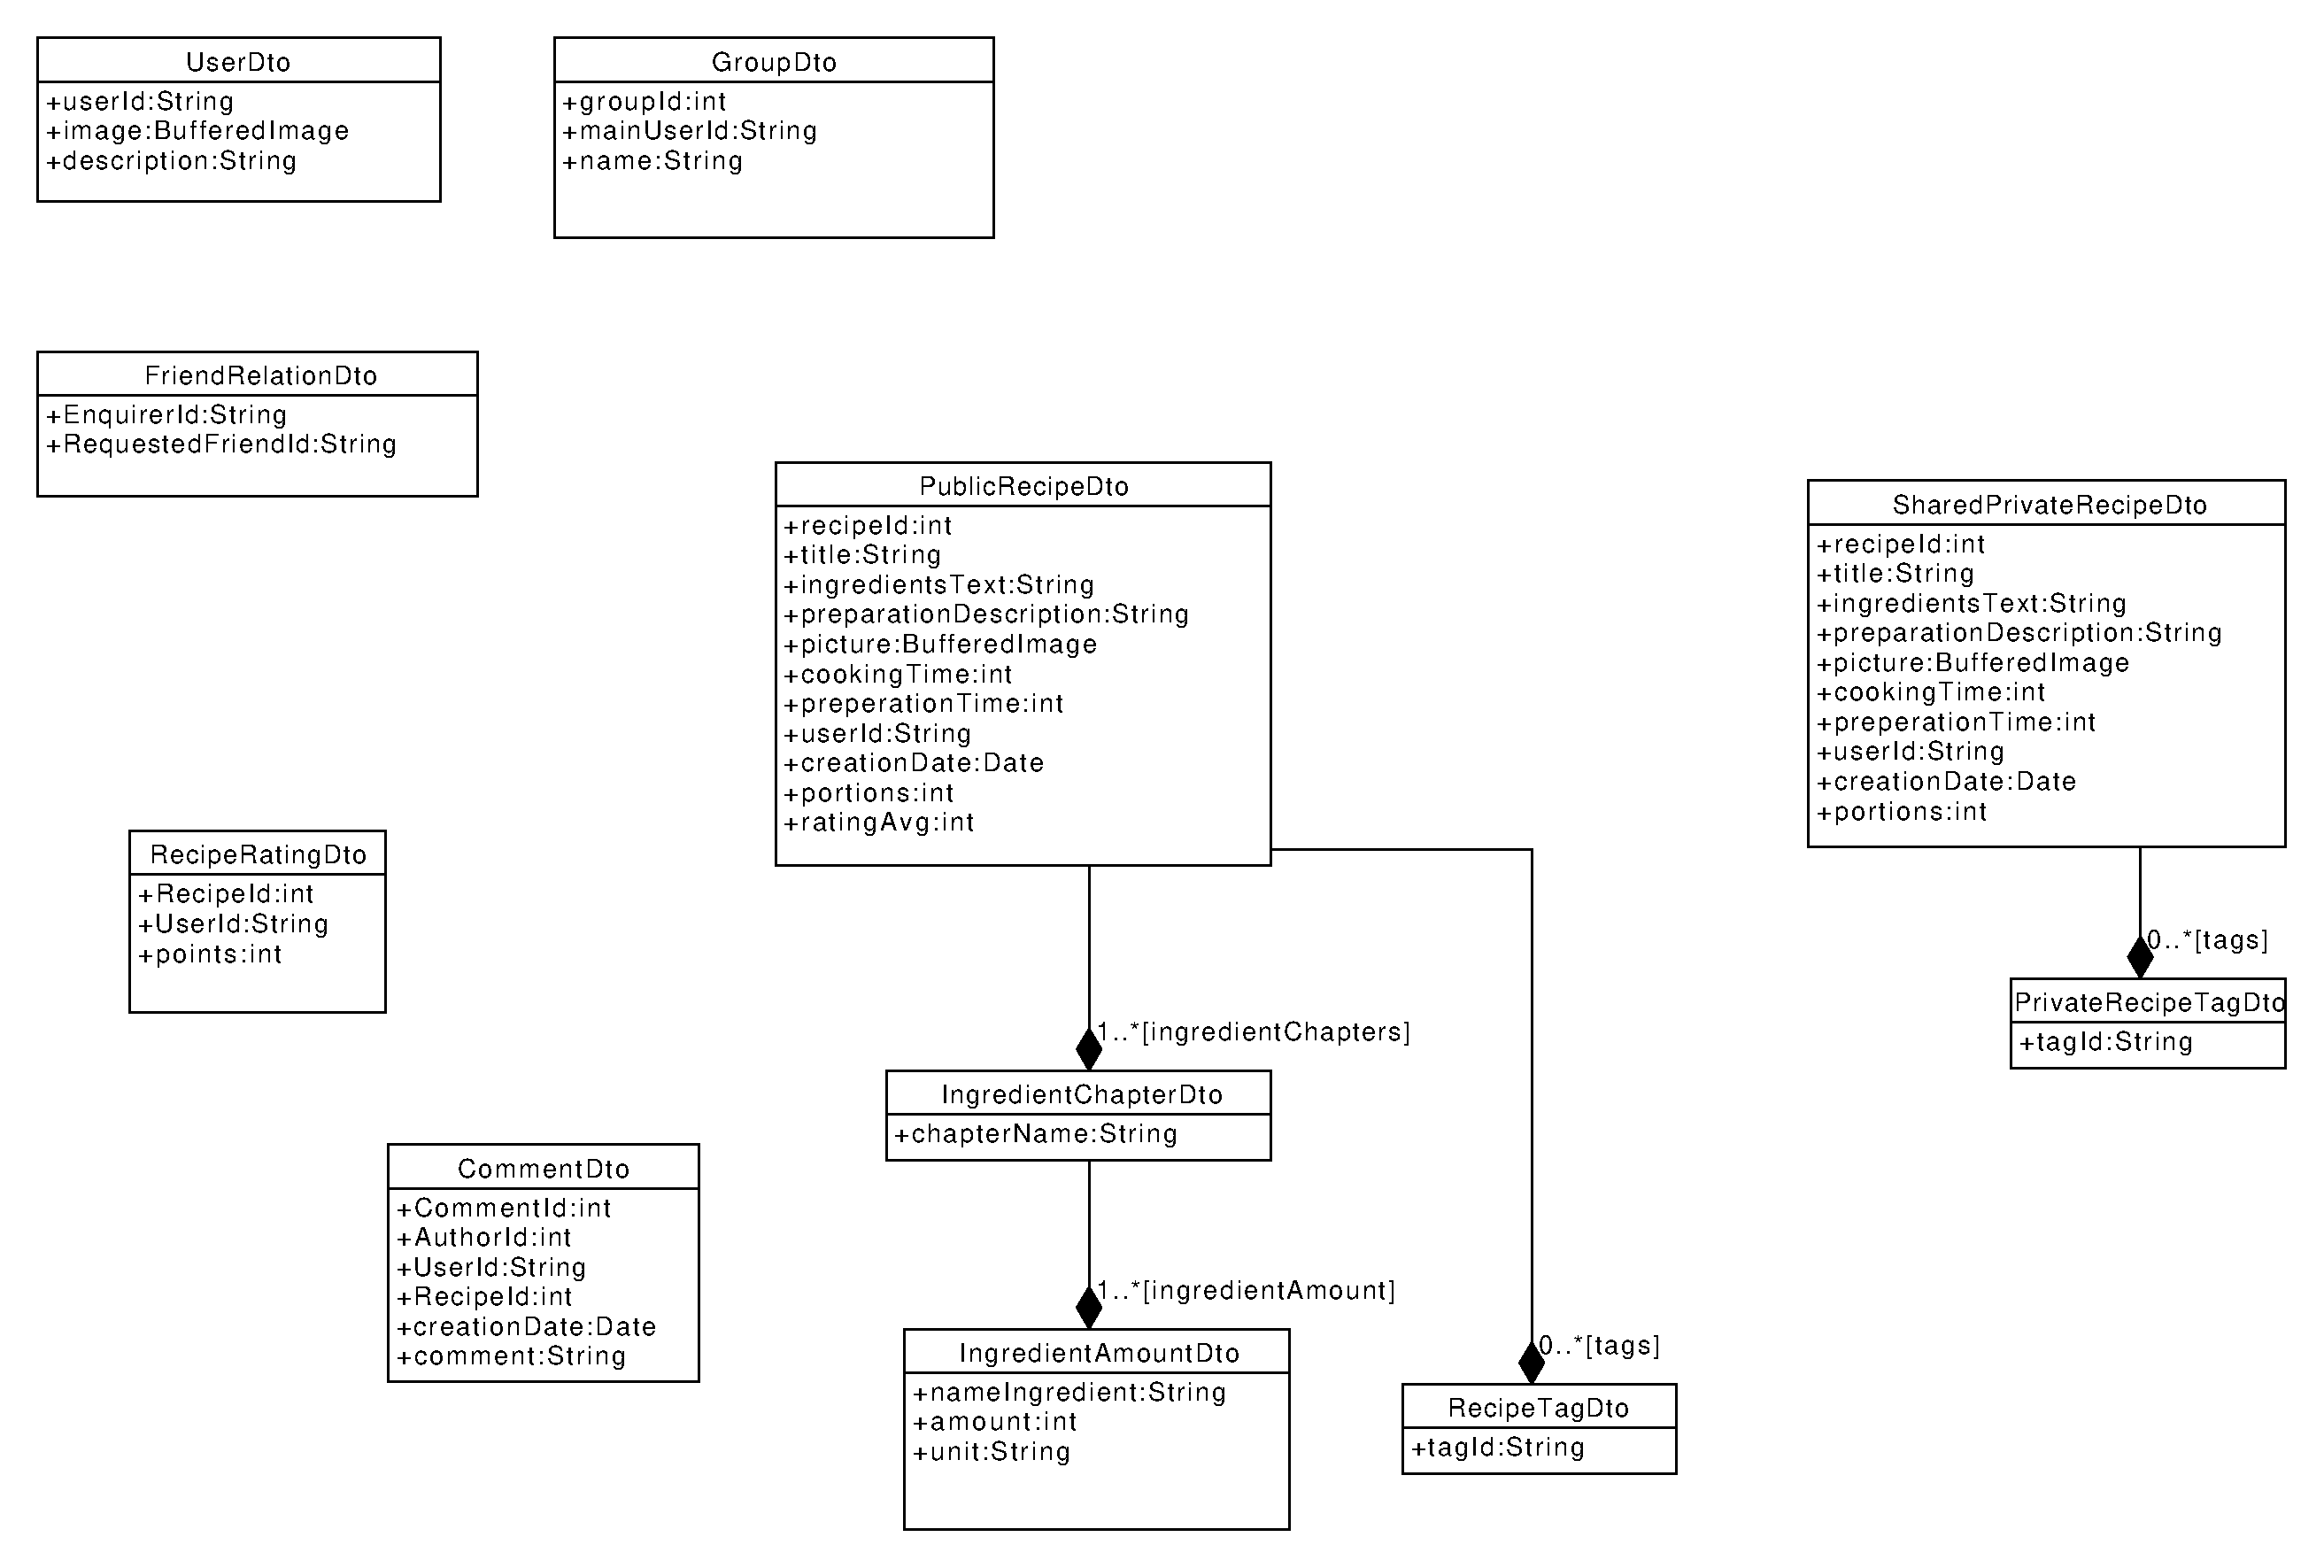
\includegraphics[width=1.0\textwidth]{generatedpics/DTO.pdf}%
	\caption{DTOs}%
	\label{dtos}
\end{figure}
Das Diagramm \ref{dtos} modelliert alle DTOs (Data transfer objects). Es ist in größerer Ansicht am ende des Dokuments erneut angefügt. Zu sehen sind Klassen, deren Hauptzweck es ist Daten zu halten. Diese Objekte, werden über die RESTschnittstelle empfangen und gesendet. 
Zur Verdeutlichung der Aggregatbeziehung im UML-Diagramm, IngredientChapters, RecipeTags und PrivateRecipeTags werden im Recipe als geschachtelte Listen versendet. Sie brauchen deswegen in der RESTschnittstelle keine gesonderte API, Comments hingegegen nicht. Sie können über eine gesonderte API gelesen und verändert werden. 

Um das anschaulicher zu machen ist unten und ein Bratapfelrezept mit drei Tags und einem seiner IngredientChapter "'Zutaten Vanillesauce"' als JSON serialisiert dargestellt:


\begin{lstlisting}[language=json]
{
  "recipeId": 3,
  "title": "Bratapfel",
  
  ...
  
  "ingredientChapters": [
    {
      "chapterName": "Zutaten Vanillesauce",
      "IngredientAmount": [
        {
          "nameIngredient": "Zucker",
          "amount": 2,
          "unit": "Essl."
        },
        {
          "nameIngredient": "Milch",
          "amount": 500,
          "unit": "Milliliter"
        }
      ]
    }
  ]
  "tags": [ "Nachtisch", "Weihnachten", "Familienklassiker" ]
}

\end{lstlisting}
